
\documentclass[linenumbers,trackchanges,twocolumn]{aastex7}

\newcommand{\vdag}{(v)^\dagger}
\newcommand\aastex{AAS\TeX}
\newcommand\latex{La\TeX}


\begin{document}

\title{Charting M33's Stellar Stream Dynamics Following The Milky Way-M31 Merger}

 

\author{Arthur Sant'Ana}
\affiliation{University of Arizona}
\email{assantana@arizona.edu}  




\begin{abstract}
    In this project I will be exploring the dynamics of stellar streams and analyzing what could be their importance in the evolution of galaxies. Stellar streams are thought to be a resulting factor of galaxy mergers, and present invaluable information on how the mass of smaller satellite galaxies may be transferred to a more massive companion, such as the timescale of such event. To accomplish the objectives in this project I will be using an N-body simulation of the MW-M31-M33 system and code developed throughout homeworks and lab assignments. The specific goal of this project is too look specifically at the velocity dispersion of stars no longer bound by M33 throughout the MW-M31 merger and how these velocity dispersions relate to their distance to the M33 center-of-mass, this will help us have a better understanding of the processes involved with tidal stripping of satellites in mergers. My first finding for this project was that as the merger goes on, not only the numbers of particles bound by M33 goes up, but also the velocity dispersion of these particles in relation to the M31 center-of-mass motion, which then seems to stabilize in a cyclical behavior pattern. My second and final finding was that, as time passes, stars no longer bound to M33 seem to present lower and lower velocity dispersion values compared to the M31 center-of-mass motion, which could indicate these objects being captured by the M31-MW system, something predicted by the $\Lambda$CDM cosmology model.
\end{abstract}


\keywords{\uat{Jacobi Radius}{} --- \uat{Tidal Stripping}{} --- \uat{Satellite Galaxy}{} --- \uat{Tidal Tails}{} --- \uat{Hierarchical Growth}{}}


\section{Introduction} \label{sec:introduction}

For the most prominent model on how galaxies evolve, the standard $\Lambda$CDM cosmology, galaxies follow a model of \textbf{hierarchical growth} and evolve via a series of mergers with neighboring smaller star systems \citep{Johnston2008-bz}, mostly via a process called \textbf{tidal stripping}, through which more massive galaxies strip smaller objects from stars and other materials by strong tidal forces. One of the predicted resulting factors in these mergers are coherent streams of stars that are stripped from their original host by the stronger tidal forces from the larger galaxy \citep{Jensen2021-mw}. These stellar streams are basically \textbf{tidal tails}, which are broad arcing arms of stars and gas, that have been more broadly spread out through the orbit of a satellite. As such, the existence of such streams hints at the scenario in which galaxies evolve via merging, and the dynamics of such objects may reveal crucial information on the history of a given galaxy.

Considering the distance these streams generally are from the galactic center, their dynamical timescales are much longer, which allows us to peer into past conditions of the system, forming something akin to a "fossil record" for past mergers of a specific galaxy \citep{Johnston1996-uv}. Thus, studying these streams' dynamics is deeply beneficial to understanding how galaxies evolve and can even provide insight on how different kinds of mergers affect the resulting galaxy, strengthening or weakening the $\Lambda$CDM framework. Furthermore, it has been discussed that measuring the amounts of stellar streams a galaxy has can put a lower limit to past merging events and also present indirect evidence for the existence of dark matter sub-haloes \citep{Malhan2018-mh}.

At this point in time, as \cite{Jensen2021-mw} evidences, we are getting access to revolutionary amounts of observational data concerning galactic structures, which includes cataloging Milky Way's stellar streams (Figure \ref{fig:general}). This revolution also comes in the form of deeply detailed simulations aiming at describing the behaviors of such streams and justifying the observations we are gathering \citep{Choi2007-lc}.

%% The "ht!" tells LaTeX to put the figure "here" first, at the "top" next
%% and to override the normal way of calculating a float position.
%% The asterisk after "figure" tells the compiler to span multiple columns
%% if a two column style is selected.
\begin{figure*}[ht!]
\epsscale{0.6}
\plotone{Stellarstream2.jpeg}
\caption{Chart demonstrating potential stream stars identified in \citep{Malhan2018-mh}. This evidences the astounding capability we have to identify these objects, however this only accounts for a small portion of all stream stars.}
\label{fig:general}
\end{figure*}


Despite the enormous advances and breakthroughs seen in recent years, big questions remain. Some depend only on our advancing observational technology, such as what the total quantity of stellar streams would be for our own galaxy, as even at this point some remain to be found \citep{Shipp2023-qz}. Others that, even with technological advancements, may still be impossible to answer completely, such as what the nature of Dark Matter is or how galaxies are created and evolve in a more detailed frame, given the presence of highly stochastic processes \citep{Amorisco2017-oc}. However, the most pressing ones for this subject relate to how the kinematics are in these streams and the process through which they end up being accreted and have their mass assimilated by more massive galaxies, making them evolve. Answering these may result in a massive jump in how well we understand stellar streams and their broader impacts on galaxy evolution. 




\section{Proposal} \label{sec:proposal}

The aim within this project is going to be to better describe the stellar streams that will originate from a \textbf{satellite galaxy}, a smaller galaxy that is bound to a larger and brighter one, throughout a major merging event. More specifically we will be looking at particle simulations of M33 during the Milky Way-M31 merger. I will be looking especially at the dynamic properties of such an event, such as the velocity dispersion in the stream and how it evolves with time. My final goal is to answer how these kinematics evolve throughout the merging process and whether or not we can draw any conclusions from its behavior that may advance current research. 

The main open question this project aims to address is how the kinematics in these streams look both in a detailed and more general frames throughout a major merging event. By understanding these kinematics better we may be able to draw some conclusions about the roles such streams play in the evolution of galaxies.

At this point in time having a better understanding of the mechanisms and timeframes that play into how galaxies evolve is extremely important for our understanding of the Universe. Be it for the construction of an accurate timeline of its past events or even theorizing what could come to happen in the far future. Understanding these "minor" mechanisms is the key.

\section{Methods} \label{sec:methods}

To achieve such goals many of the functions devised during classes and labs will be used, which include a N-body simulation of the collision between M31 and the Milky Way \citep{Van_der_Marel2012-bf}. First the relevant snap shots from the simulation will be selected. In this case snap shots before and after each MW-M31 interaction will be the most useful, so around 3.8 Gyr ("M33$\_$260.txt"), 5.9 Gyr ({"M33$\_$420"}) and beyond 6.5 Gyr ("M33$\_$460"). Since stars are being addressed, only disk particles will be used. These points of interest can be clearly seen using the separation plot devised in Homework 6.


Now we have to find which particles are not bound to M33 at each of these moments. In order to do that we will be using the \textbf{Jacobi Radius}, which is defined as:

\begin{equation}
    R_j = r*{(\frac{M_{sat}}{2M_{host}(<r)})}^{\frac{1}{3}}
\end{equation}

This equation takes in the mass of the satellite M33 ($M_{sat}$), the mass of the host MW+M31 ($M_{host}$) (only the mass sitting in between the center of mass and the satellite are accounted for at any moment) and $r$, which is the separation between these two.

Both masses can be easily obtained directly from the "GalaxyMass.py" function created in Homework 3. The separation, however, will require some extra steps. The base code will come from Homework 6, where we used the "CenterOfMass" class and created the "orbitCOM" function in order to plot the separation between each object in terms of time. For this project we will be using "orbitCOM" in order to obtain the separation for a given time and plugging that into the Jacobi Radius formula.

Then finally we will be able to use the code developed on Lab 7 to make plots for the velocity dispersion compared to the M31 center-of-mass frame. The Jacobi radius will be used as a condition, so only particles beyond the Jacobi radius will be shown in the plots, allowing us to clearly see the characteristics and how they change from time to time during the merging event. See Figure \ref{fig:general2} for reference. Furthermore I will also be plotting the velocity dispersion throughout time, and how the values change for it during the merger. Another plot that can be devised is one that looks at how the velocity dispersion changes for particles in terms of how far away they are from the M33 center-of-mass. These plots will all be deeply meaningful in understanding the dynamics in these streams and what observational data could expect from such events.

\begin{figure}
    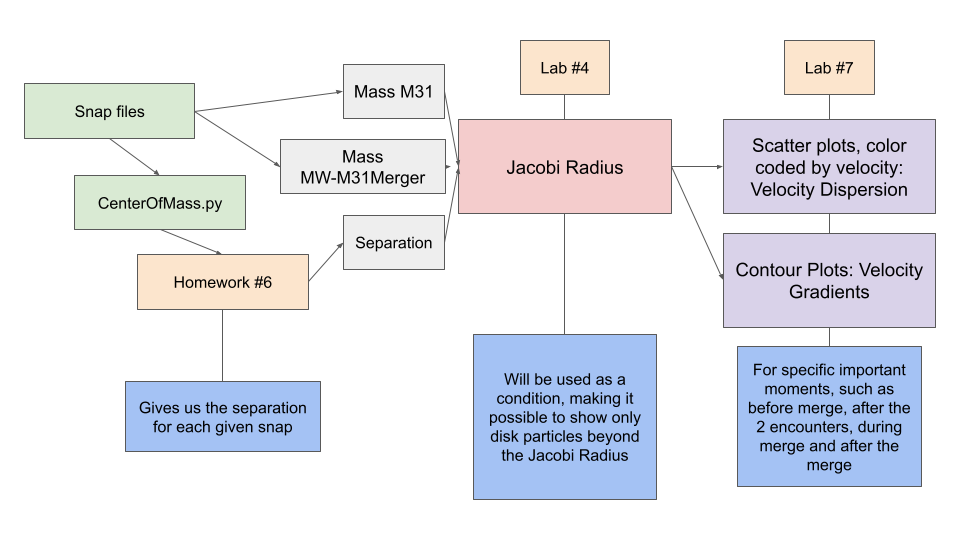
\includegraphics[width=\linewidth]{DiagramRA.png}
    \caption{Diagram illustrating the steps that need to be taken in order to obtain velocity dispersion and gradient plots of particles located beyond the Jacobi radius (No longer bound by M33). In blue we can see more detailed explanations for how each function developed during an assignment will be used.
    \label{fig:general2}}
\end{figure}


\subsection{Hyposthesis}

I believe that, as the merging event advances, M33 will lose a large amount of the particles localized at its edges, most of it during the major encounters of MW and M31, since its Jacobi radius will decrease since now both MW and M31 masses are exerting tidal forces. This will probably also mean that we will see more extreme velocities beyond the Jacobi radius during those timeframes. Another prediction we can make is that as time passes these streams will slowly be accreted by the now merged MW-M31 system, since this is what the $\Lambda$CDM model predicts.

\section{Results} \label{sec:results}

The first figure created in this project (Figure \ref{fig:general3}) is a plot of the mean velocity dispersion vs. time for particles beyond the Jacobi radius of M33. This plot aims at demonstrating how the velocity dispersion for stream particles in relation to the velocity of the M31 center-of-mass frame evolves throughout the merging event. The main takeaway from this plot is that overall the velocity dispersion grows rapidly during the merging event, and at the rightmost part we can start to see some sort of cyclical behavior in that dispersion, which seems to diminish in amplitude over time. Other information that can be extracted from this plot are the peaks for this velocity dispersion, which could have a deeper meaning associated.

\begin{figure}
    \centering
    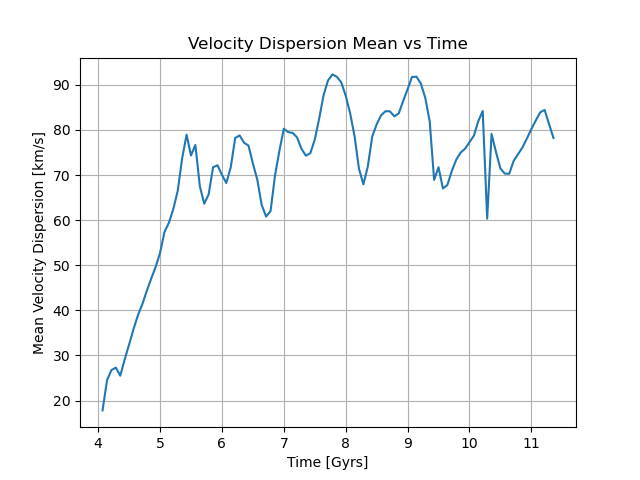
\includegraphics[width=\linewidth]{dispersion_vs_time.png}
    \caption{Plot demonstrating how the mean velocity dispersion of the stellar streams with respect to the M31 center-of-mass frame evolve throughout the collision of M31 and MW. With the mean velocity dispersion with respect to the M31 center-of-mass motion plotted on the y-axis and time on the x-axis. We can clearly see how the velocity dispersion for the stellar streams grows as the merger continues to happen.}
    \label{fig:general3}
\end{figure}

The second figure generated for this project (Figure \ref{fig:general4}) is a series of velocity dispersion versus radial distance plots, each for a given time during the merging event. The velocity dispersion in these plots is calculated with respect to the M31 center-of-mass frame. The main objective of this plot is to portray the velocity dispersion profile of the stellar streams at some points in time during the merger. One of the takeaways of these plots is how the dispersion values for particles closer to the M33 center-of-mass grow with time, but particles further away seem to have a small velocity dispersion to the M31 center-of-mass motion.

\begin{figure}
    \centering
    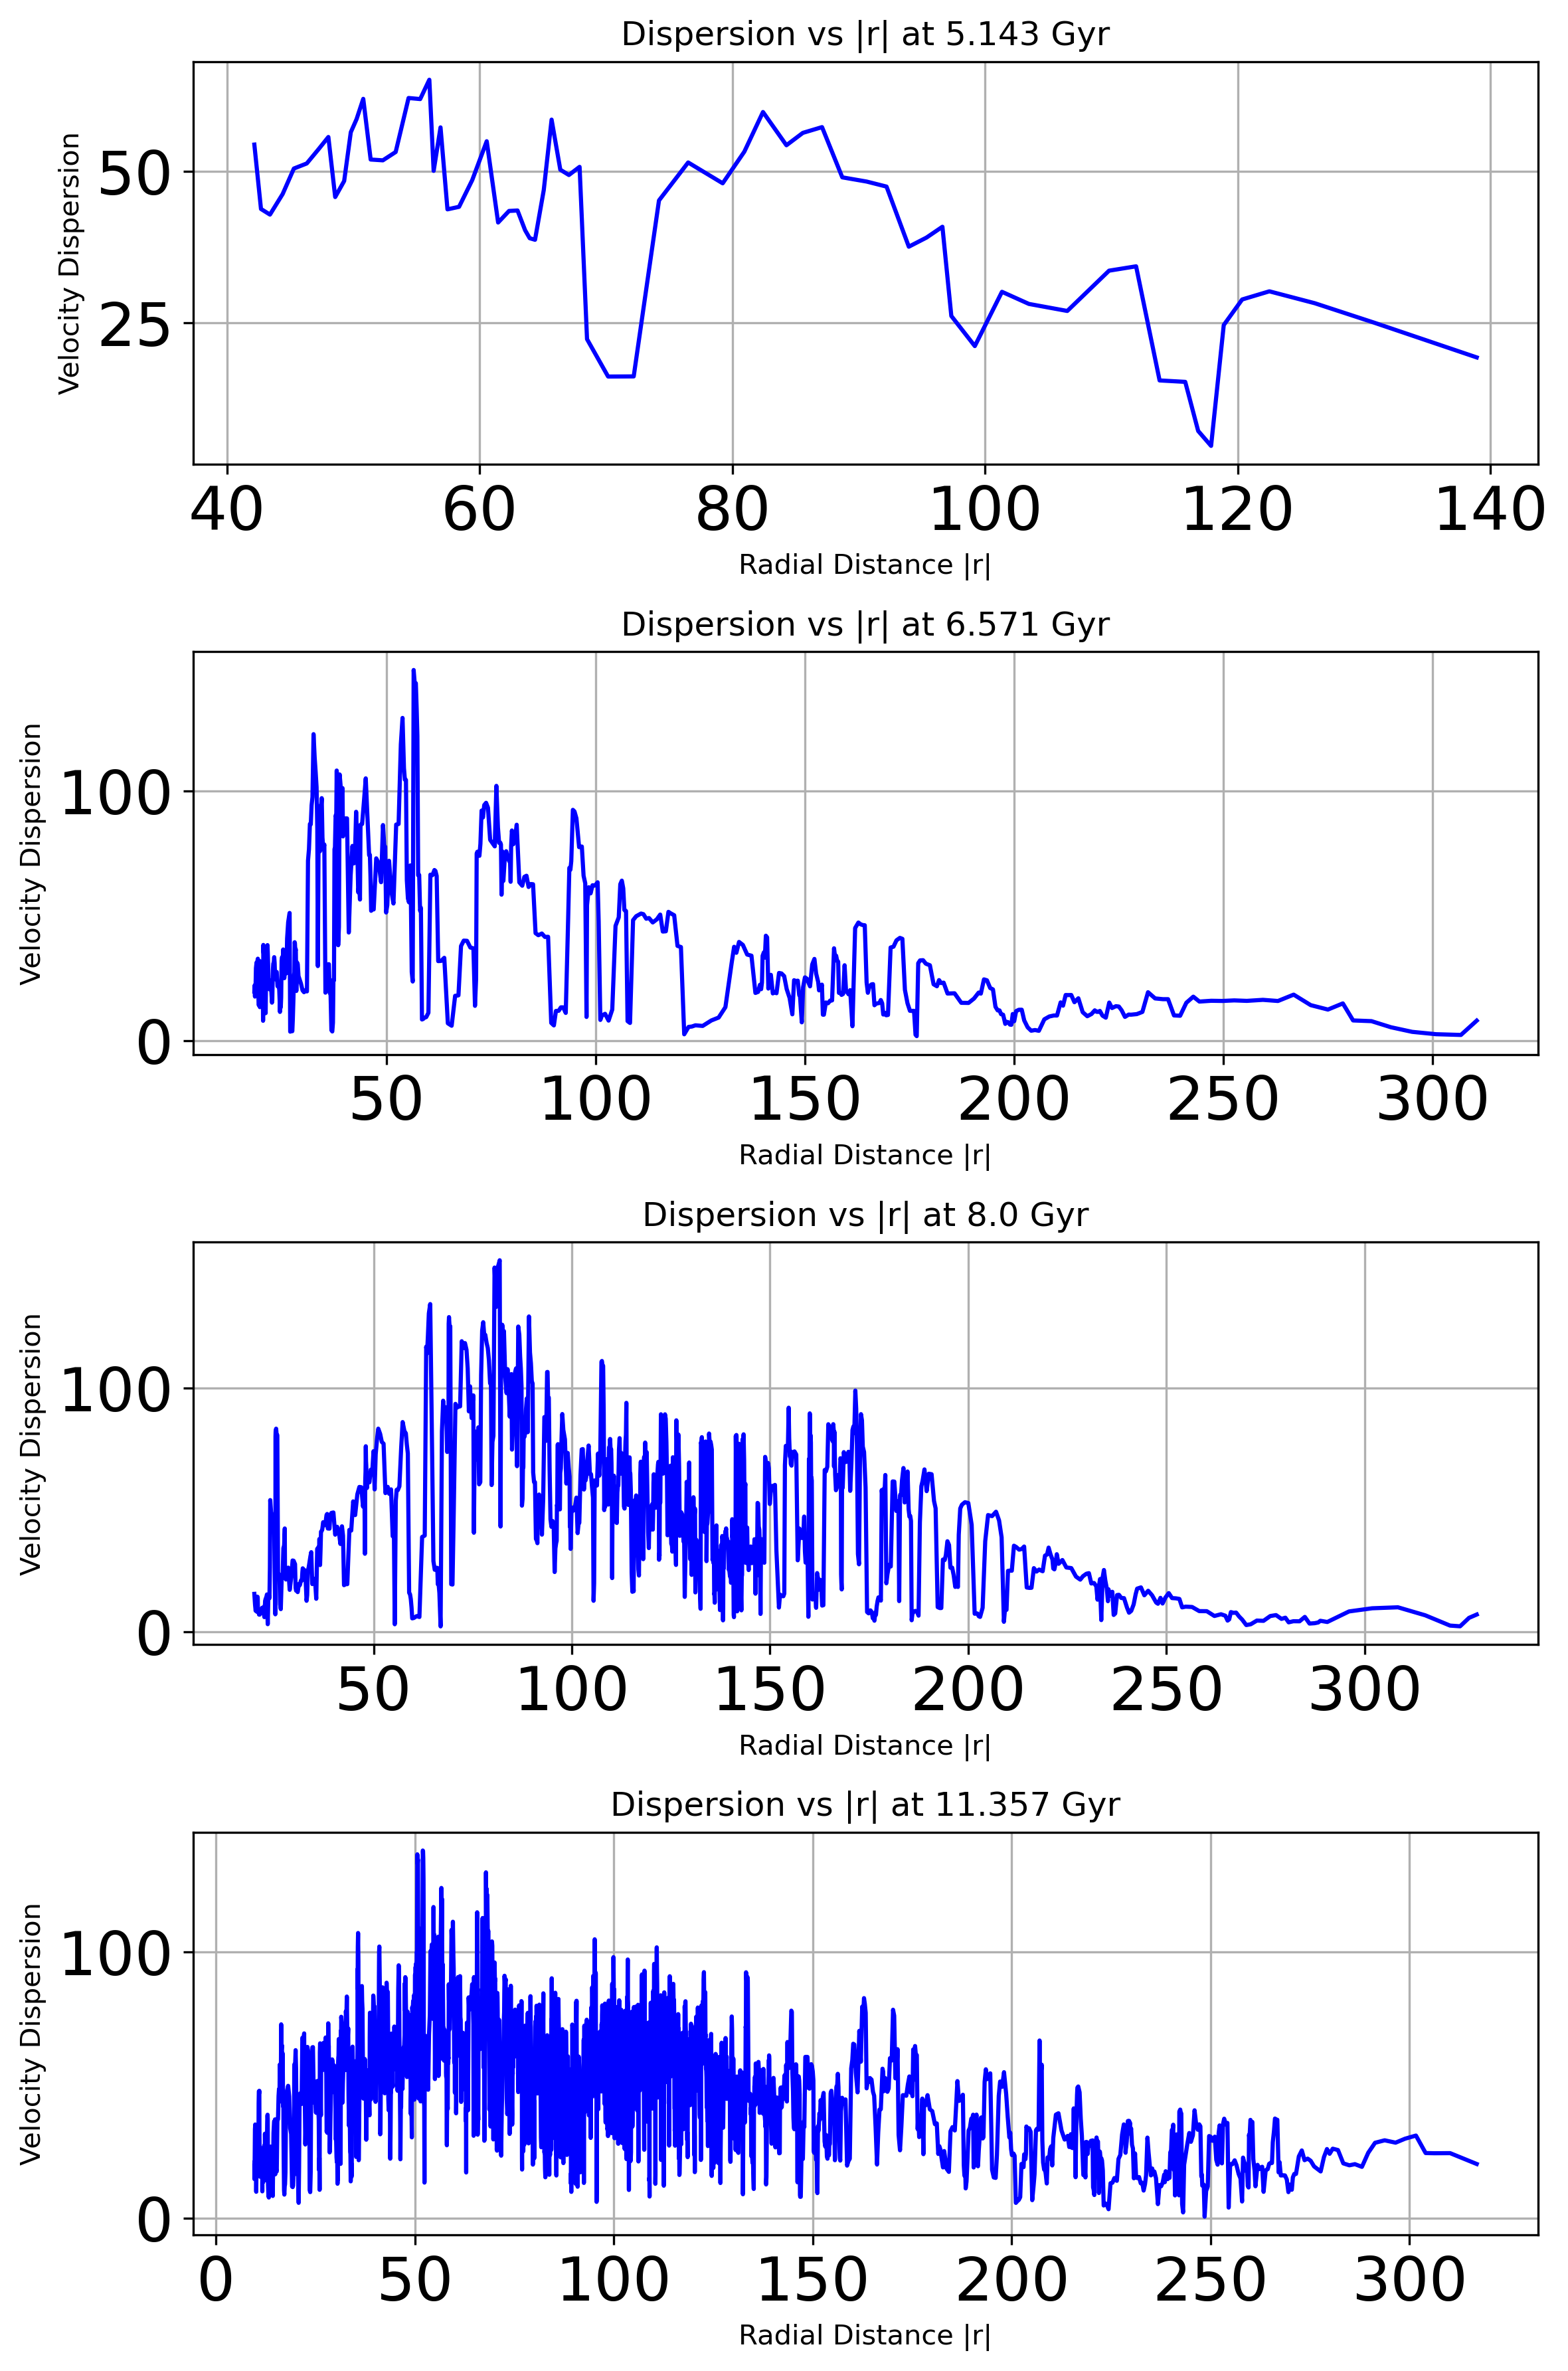
\includegraphics[width=\linewidth]{dispersion_vs_radius.png}
    \caption{Plot demonstrating how the velocity dispersion looks like for different radii at key moments in time during the merger. Velocity dispersion is plotted in the y-axis and position (radius) in the x-axis. We can see some trends in the velocity dispersion profile, such as how the maximum values grow with time, and also where the regions with the most velocity dispersion are located at a given time}
    \label{fig:general4}
\end{figure}


 

\section{Discussion} \label{sec:discussion}

The first result that can be extracted from both Figure \ref{fig:general3} and Figure \ref{fig:general4} is that the velocity dispersion increases over time, as does the number of particles classified as stream particles. Both observations are consistent with my initial broad hypothesis. However, we now obtain even more detailed information, such as the dispersion profile, which allows for a deeper analysis of stellar streams.

The simulations conducted by \cite{Choi2007-lc} provide valuable insight into the structure of these streams under various scenarios. A key observation is that, over time, more particles leave the satellite and travel progressively farther from it, an effect that is also evident in my results. However, \cite{Choi2007-lc} focuses on the density and spatial distribution of the streams and does not examine their velocity dispersion. My results may therefore complement the simulation-based research on stellar streams by providing data on the velocities associated with this phenomenon and how they relate to the distance from the satellite.

A significant source of uncertainty—and indeed a limitation—in my analysis is the evolving mass profile of the MW–M31 system, which alters the Jacobi Radius of M33 in ways that my code does not currently account for. As a result, any conclusions drawn from the plots will inherently contain some degree of uncertainty in terms of the absolute Jacobi radius at a given moment. This, in turn, affects the classification of particles as stellar stream members. However, this limitation does not affect the overall shape of the mean velocity dispersion curves shown in Figure \ref{fig:general3} and Figure \ref{fig:general4}; any discrepancies could be addressed by applying a shift along the x-axis to adjust for the changing Jacobi radius.

Another notable finding from my project is that, long after the onset of the merger, the velocity dispersion of stellar stream particles appears to present a sinusoidal behavior with the apparent amplitude going down with time(Figure \ref{fig:general3}). This trend may reflect the process by which these particles become assimilated into the newly formed MW–M31 merged galaxy. Supporting this idea, Figure \ref{fig:general4} shows that velocity dispersions at higher distances tend to be smaller than the ones closer to the M33 center-of-mass as time passes, such that the farthest particles exhibit lower dispersions in the last snapshot used than seen at previous snapshots, meaning they have a dispersion more similar to that of the M31 center-of-mass than the rest of the detached particles. Additionally, the spatial extent of the stream increases over time, with its outer boundary expanding from 24 kpc at the beginning to 300 kpc in the final snapshot.

These findings are consistent with the $\Lambda$CDM model and predictions from \cite{Jensen2021-mw}, which suggest that stellar streams serve as a mechanism through which larger galaxies accrete material from smaller ones. Figures \ref{fig:general3} and \ref{fig:general4} offer valuable insight into the kinematic behavior of these particles after detachment from their original satellite, illustrating how their velocities evolve as they are stripped away. This information not only enhances our understanding of the final velocities of these particles as they approach the larger galaxy, but also enables estimation of the relevant timescales for these events.

The uncertainties affecting this result are largely the same as those discussed earlier. While the overall profiles remain valid, a correction factor must be introduced to adjust the location of the Jacobi Radius in order to achieve the most accurate results. Adding up to that we also have some properties of how stellar streams organize in space that make it somewhat difficult to interpret what these features seen in velocity dispersion plots mean. One of these features is the presence of a leading and trailing component to the stream, which can be seen clearly in the plots devised by \cite{Choi2007-lc}. This makes interpreting the mean of the velocity dispersion very difficult to interpret, but by using the M31 center-of-mass frame for the computation of the velocity dispersion the results seem to present a better description of the event.

\section{Conclusions}\label{sec:conclusions}

In this project I have explored the dynamics of stellar streams and analyzing what could be their importance in the evolution of galaxies. Stellar streams are thought to be a resulting factor of galaxy mergers, and present invaluable information on how the mass of smaller satellite galaxies may be transferred to a more massive companion, such as the timescale of such event. To accomplish the objectives in this project I will be using an N-body simulation of the MW-M31-M33 system and code developed throughout homeworks and lab assignments. The specific goal of this project is too look specifically at the velocity dispersion of stars no longer bound by M33 throughout the MW-M31 merger and how these velocity dispersions relate to their distance to the M33 center-of-mass, this will help us have a better understanding of the processes involved with tidal stripping of satellites in mergers.

My first finding relates to how as time passes for the merger event, the number of particles now beyond the Jacobi radius, so not a part of M33 anymore, grows. This finding is a very expected outcome and can be seen in the work done by \cite{Choi2007-lc} with stream star simulation, still having results that confirm previous work in the field is also valuable. This was generally predicted by my hypothesis, but with the plots devised we get much more information than only how the number of particles beyond the Jacobi radius grows, which leads us to my second result.

My second finding for this project pertains to how throughout time the overall mean velocity dispersion with respect to the M31 center-of-mass motion grows, until it reaches a point where it stagnates and seems to show a sinusoidal behavior with a decreasing amplitude over time. This finding is very interesting because the final behavior may be related to how these particles are expected to be part of the MW-M31 system now, more specifically part of its stellar halo. If this is the case then this trend is a very important finding to getting a better grasp at the dynamics that factor into galaxy hierarchical growth. This closely matches what I had as my hypothesis, but it expands a lot more on how we can analyze more details about the behavior of detached particles as they now assimilate to the MW-M31 system.

Despite the insights gained, this study remains limited in both accuracy and broader relevance. As noted earlier, several improvements are necessary to enhance the numerical precision of the results. One key improvement would be to incorporate the evolving dynamics of the MW–M31 center-of-mass frame during the merger, as this would influence both the Jacobi radius and the calculated velocity dispersions. Additionally, implementing a method to distinguish between the leading and trailing arms of the stellar streams—and analyzing their velocity dispersions separately—could yield a clearer understanding of their distinct behaviors. In terms of contextual relevance, producing a plot akin to Figure \ref{fig:general4}, but showing the distance of stream particles to the MW–M31 center-of-mass, could offer valuable insight into how these particles integrate into the resulting stellar halo. These enhancements would significantly elevate the quality and impact of this work.

\section{Acknowledgements}\label{sec:acknowledgements}
1. Astropy (Astropy Collaboration et al. 2013; Price-Whelan et al. 2018 doi: 10.3847/1538-
3881/aabc4f)

2. matplotlib Hunter (2007),DOI: 10.1109/MCSE.2007.55

3. numpy van der Walt et al. (2011), DOI: 10.1109/MCSE.2011.37

4. scipy Jones et al. (2001–),Open source scientific tools for Python. http://www.scipy.org/

5. ipython Perez \& Granger (2007), DOI: 10.1109/MCSE.2007.53

6. ChatGPT(22 Apr. version) OpenAI(2023) "I have an array of velocities in this format vJ = ([vx,vy,vz]), how would I make a graph of the dispersion of these velocities vs time?" prompt, chat.openai.com/chat



\newpage
\bibliography{BibResearchAssi2}{}
\bibliographystyle{aasjournalv7}



\end{document}


